\doublespacing % Do not change - required

\chapter{How To ...... in\LaTeX ?}
\label{chHT}

%%%%%%%%%%%%%%%%%%%%%%%%%%%%%%%%%%%%%%%
% IMPORTANT
\begin{spacing}{1} %THESE FOUR
\minitoc % LINES MUST APPEAR IN
\end{spacing} % EVERY
\thesisspacing % CHAPTER
% COPY THEM IN ANY NEW CHAPTER
%%%%%%%%%%%%%%%%%%%%%%%%%%%%%%%%%%%%%%%

{\color{red}This section provides detailed examples of equations, tables, figures, etc. that you will use in LATEX to help you with your interim and final reports. Please review the recommended websites!!!!!!!}

\section{Introduction}

In this section, some crucial point about how to fill this template are given such as formulation, figures, tables etc.

\section{How to define an equation ?}
\medskip
A simple and a complex examples are given in equation (\ref{eq:simpleexample}) and equation (\ref{eq:complexexample})

\begin{equation}
    u(t) = K_p e \left( t\right) + K_i \int_0^t \left( \tau\right) dt + K_d \frac{d e \left( t\right)}{dt}
    \label{eq:simpleexample}
\end{equation}

%
%
\begin{equation}
\begin{split}
& \mathbf{F_1}=\{i \ | \ |\beta_i|=Z, |G\left(\mathbf{x_i}\right)|\geq \epsilon \} \\
& \mathbf{F_2}=\{i \ | \ 0< |\alpha_i|<P, |G_2\left(\mathbf{x_{ijkl}}\right)|=0  \} \\ 
& \mathbf{\omega_{PSA}}=\{k \ | \ |\lambda_i|=0, | \phi\left(\mathbf{x_i}\right)|\leq \varepsilon  \}
\end{split}
\label{eq:complexexample}
\end{equation}
%
%
For more detailed informations, you can use \url{https://www.overleaf.com/learn/latex/Mathematical_expressions} and "Further reading" sections given in previous website.
%
%
\subsection{How to define matrix?}


\begin{equation}
\boldsymbol{\Omega}=\begin{bmatrix}
	\Omega_{s_0}\\
	\Omega_{s_1}\\
	\vdots\\
	\Omega_{s_k}
	\end{bmatrix} =-\mathbf{\Theta}\begin{bmatrix}
	1\\
	2\\
	\vdots\\
	K
	\end{bmatrix} \ , \
	\label{eq:10}
\end{equation}


\begin{equation}
%\begin{split}
\boldsymbol{\Omega}=\begin{bmatrix}
	\Omega_{s_0}\\
	\Omega_{s_1}\\
	\vdots\\
	\Omega_{s_k}
	\end{bmatrix} =-\mathbf{\theta}\begin{bmatrix}
	1\\
	2\\
	\vdots\\
	K
	\end{bmatrix} \ , \
    	\mathbf{\theta}=\begin{bmatrix}
	\theta_{11} & \theta_{12} & \cdots &\theta_{1k} \\
	\theta_{21} & \theta_{22} & \cdots &\theta_{2k} \\
	\vdots & \vdots & \ddots & \vdots \\
    \theta_{k1} & \theta_{k2} & \cdots &\theta_{kk}
	\end{bmatrix}^{-1}
%\end{split}        
	\label{eq:10}
\end{equation}
%
%






\subsection{How to split Long equations?}

You can use "split" command given as below:

\begin{equation}
\begin{split}
&\boldsymbol{\Omega}=\begin{bmatrix}
	\Omega_{s_0}\\
	\Omega_{s_1}\\
	\vdots\\
	\Omega_{s_k}
	\end{bmatrix} =-\mathbf{\theta}\begin{bmatrix}
	1\\
	2\\
	\vdots\\
	K
	\end{bmatrix} \ , \\
    &
    	\mathbf{\theta}=\begin{bmatrix}
	\theta_{11} & \theta_{12} & \cdots &\theta_{1k} \\
	\theta_{21} & \theta_{22} & \cdots &\theta_{2k} \\
	\vdots & \vdots & \ddots & \vdots \\
    \theta_{k1} & \theta_{k2} & \cdots &\theta_{kk}
	\end{bmatrix}^{-1}
\end{split}        
	\label{eq:10}
\end{equation}

%
%
For detailed information you can use the following website.

\medskip
For detailed information you can use the following website.\\
\url{https://www.overleaf.com/learn/latex/Aligning_equations_with_amsmath}


\subsection{Significant Greek Symbols utilized in \LaTeX}

Some symbols are given below



In addition to these, you can find much more detailed information on the website below. In addition, LLM structures will be very helpful.

\begin{itemize}
\item \url{https://www.overleaf.com/learn/latex/List_of_Greek_letters_and_math_symbols}
\item \url{https://ftp.cc.uoc.gr/mirrors/CTAN/info/symbols/comprehensive/symbols-a4.pdf}
\item \url{https://www.geeksforgeeks.org/greek-alphabet-symbols/}

\item Your LLM Friends(ChatGPT, Deepseek etc) 
\end{itemize}


\subsubsection{Greek Alphabet}
\subsubsection{Lowercase Letters}
\begin{tabular}{ll | ll | ll}
\textbackslash alpha & $\alpha$ & \textbackslash nu & $\nu$ & \textbackslash upsilon & $\upsilon$ \\
\textbackslash beta & $\beta$ & \textbackslash xi & $\xi$ & \textbackslash phi & $\phi$ \\
\textbackslash gamma & $\gamma$ & \textbackslash omicron & $o$ & \textbackslash chi & $\chi$ \\
\textbackslash delta & $\delta$ & \textbackslash pi & $\pi$ & \textbackslash psi & $\psi$ \\
\textbackslash epsilon & $\epsilon$ & \textbackslash rho & $\rho$ & \textbackslash omega & $\omega$ \\
\textbackslash zeta & $\zeta$ & \textbackslash sigma & $\sigma$ &  &  \\
\textbackslash eta & $\eta$ & \textbackslash tau & $\tau$ &  &  \\
\textbackslash theta & $\theta$ & \textbackslash iota & $\iota$ &  &  \\
\end{tabular}

\subsubsection{Uppercase Letters}
\begin{tabular}{ll | ll | ll}
\textbackslash Gamma & $\Gamma$ & \textbackslash Lambda & $\Lambda$ & \textbackslash Sigma & $\Sigma$ \\
\textbackslash Delta & $\Delta$ & \textbackslash Xi & $\Xi$ & \textbackslash Upsilon & $\Upsilon$ \\
\textbackslash Theta & $\Theta$ & \textbackslash Pi & $\Pi$ & \textbackslash Phi & $\Phi$ \\
\textbackslash Omega & $\Omega$ & \textbackslash Psi & $\Psi$ &  &  \\
\end{tabular}

\subsubsection{Mathematical Symbols}
\subsubsection{Commonly Used Symbols}
\begin{tabular}{ll | ll | ll}
\textbackslash infty & $\infty$ & \textbackslash pm & $\pm$ & \textbackslash times & $\times$ \\
\textbackslash sum & $\sum$ & \textbackslash prod & $\prod$ & \textbackslash int & $\int$ \\
\textbackslash sqrt & $\sqrt{x}$ & \textbackslash frac & $\frac{a}{b}$ & \textbackslash lim & $\lim$ \\
\textbackslash sin & $\sin x$ & \textbackslash cos & $\cos x$ & \textbackslash tan & $\tan x$ \\
\textbackslash log & $\log x$ & \textbackslash exp & $\exp x$ & \textbackslash ln & $\ln x$ \\
\end{tabular}

\subsubsection{Relational Symbols}
\begin{tabular}{ll | ll | ll}
\textbackslash leq & $\leq$ & \textbackslash geq & $\geq$ & \textbackslash neq & $\neq$ \\
\textbackslash approx & $\approx$ & \textbackslash equiv & $\equiv$ & \textbackslash subset & $\subset$ \\
\textbackslash supset & $\supset$ & \textbackslash subseteq & $\subseteq$ & \textbackslash supseteq & $\supseteq$ \\
\end{tabular}

\subsubsection{Logic and Set Notation}
\begin{tabular}{ll | ll | ll}
\textbackslash forall & $\forall$ & \textbackslash exists & $\exists$ & \textbackslash neg & $\neg$ \\
\textbackslash in & $\in$ & \textbackslash notin & $\notin$ & \textbackslash emptyset & $\emptyset$ \\
\textbackslash cap & $\cap$ & \textbackslash cup & $\cup$ & \textbackslash subseteq & $\subseteq$ \\
\textbackslash wedge & $\wedge$ & \textbackslash vee & $\vee$ & \textbackslash Rightarrow & $\Rightarrow$ \\
\textbackslash Leftrightarrow & $\Leftrightarrow$ & \textbackslash bot & $\bot$ & \textbackslash top & $\top$ \\
\end{tabular}

\subsubsection{Brackets and Parentheses in Mathematical Expressions}
The following web site will help you for detailed information about Brackets and Parentheses " 
\url{https://www.overleaf.com/learn/latex/Brackets_and_Parentheses} " .




















\section{How to upload Figure etc?}


\begin{figure}
\centering
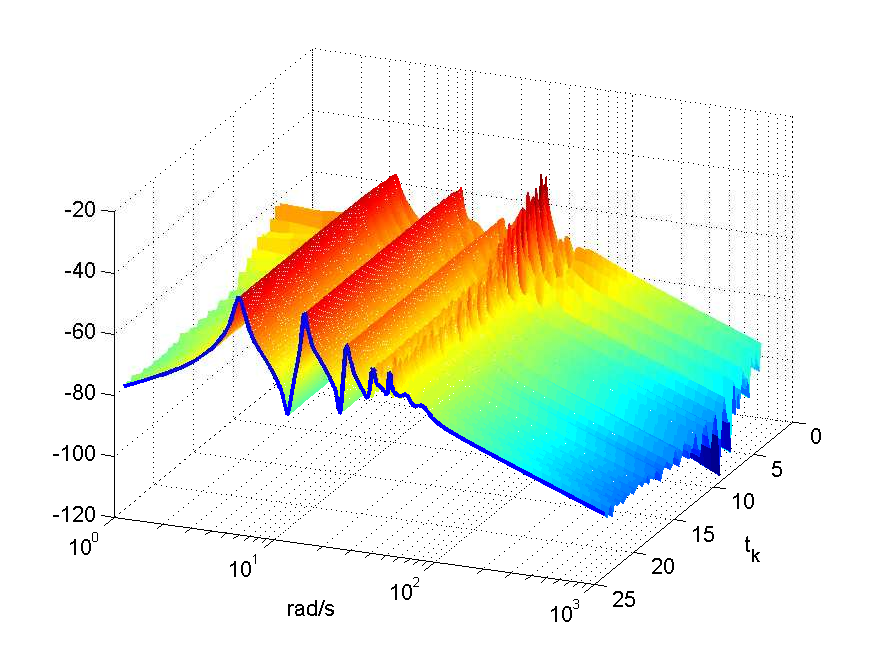
\includegraphics[width=0.8\columnwidth]{imgs/buildmagnitude.pdf}
\caption[Short description for list of figures]{This figure is taken from \cite{Sca:16}.}
\label{fig-magnitude}
\end{figure}%




\section{How to define Tables?}


In this section tables, equation etc examples are given. As given in Table~\ref{tab:1}, xxxxxxxxxx can be.

\begin{table*}[htbp]
	\caption{Comparison of Various Methods.}
	\begin{center}
		\begin{tabular}{l l l l l l l}
			%\hline
			%\multicolumn{7}{c}{Computation Times(in ms) for controllers} \\
			\cline{1-7}
			%Systems&&  IP System\\
			\hline
             Methods &  & Method 1&  &  & Method 2& \\
			\cline{1-7}
			Operations $\setminus$ Cases & Case 1& Case 2& Case 3 & Case 1 & Case 2 & Case 3\\
			\hline
			Operation 1 & 0.93684	&0.89219	&1.5028	&1.2275 &2.6182	&1.1922\\
            Operation 2 & 0.053503	&0.061289	&0.049883	&0.038601 &0.045261	&0.039763\\
            Operation 3 & 0.20027	&0.63789	&0.20335	&0.19014 &1.6918	&0.19196\\
            Operation 4 &0.28225	&0.40756	&0.32971	&0.24073 &0.3323	&0.2559\\
            Operation Final &1.4729	&1.9989	&2.0857  &1.6969 &4.6875	&1.6798\\
			\hline
		\end{tabular}
	\end{center}
	% \caption{Computation Times(in ms) for controllers}
	\label{tab:1}
\end{table*}
%
%



\section{How to define Algorithms and depict Flowcharts?}
An example for a pseudo code is given below. In order to cite an algorithm don't forget to label your algorithms such as "$\text{\label{alg:1}}$" . Algorithm~\ref{alg:1} is given below :
\begin{algorithm}
\caption{An algorithm with caption}\label{alg:1}
\begin{algorithmic}
\Require $n \geq 0$
\Ensure $y = x^n$
\State $y \gets 1$
\State $X \gets x$
\State $N \gets n$
\While{$N \neq 0$}
\If{$N$ is even}
    \State $X \gets X \times X$
    \State $N \gets \frac{N}{2}$  \Comment{This is a comment}
\ElsIf{$N$ is odd}
    \State $y \gets y \times X$
    \State $N \gets N - 1$
\EndIf
\EndWhile
\end{algorithmic}
\end{algorithm}

You can reach comprehensive information about Alogirthms etc via \url{https://www.overleaf.com/learn/latex/Algorithms}

Flow chart detailed informations are here \url{https://www.overleaf.com/learn/latex/LaTeX_Graphics_using_TikZ%3A_A_Tutorial_for_Beginners_(Part_3)%E2%80%94Creating_Flowcharts}



\tikzstyle{startstop} = [rectangle, rounded corners, 
minimum width=3cm, 
minimum height=1cm,
text centered, 
draw=black, 
fill=red!30]

\tikzstyle{io} = [trapezium, 
trapezium stretches=true, % A later addition
trapezium left angle=70, 
trapezium right angle=110, 
minimum width=3cm, 
minimum height=1cm, text centered, 
draw=black, fill=blue!30]

\tikzstyle{process} = [rectangle, 
minimum width=3cm, 
minimum height=1cm, 
text centered, 
text width=3cm, 
draw=black, 
fill=orange!30]

\tikzstyle{decision} = [diamond, 
minimum width=3cm, 
minimum height=1cm, 
text centered, 
draw=black, 
fill=green!30]
\tikzstyle{arrow} = [thick,->,>=stealth]


 \begin{tikzpicture}
        \node (start) [startstop] {Start};
        \node (input) [process, below of=start, yshift=-1.5cm] {Enter exam score};
        \node (decision) [decision, below of=input, yshift=-2cm] {Score >= 50?};
        \node (pass) [process, right of=decision, xshift=4cm] {Pass};
        \node (fail) [process, below of=decision, yshift=-2cm] {Fail};
        \node (end) [startstop, below of=fail, yshift=-1.5cm] {End};
        
        \draw [arrow] (start) -- (input);
        \draw [arrow] (input) -- (decision);
        \draw [arrow] (decision.east) -- node[anchor=south] {Yes} (pass.west);
        \draw [arrow] (pass.south) |- (end.east);
        \draw [arrow] (decision.south) -- node[anchor=east] {No} (fail.north);
        \draw [arrow] (fail.south) -- (end.north);
        
\end{tikzpicture}
    
\section{How to add ..... in Text?}
\subsection{How to add footnotes?}

Start writing your suggestions section here.\footnote{This is an example of footnote usage!}

\subsection{How to add Mathematical Expression in TEXT?}
You can add mathematical expression in text by definig expression inside two "\$". An axmple can be considered as $\sum_{i=1}^{\infty}\frac{1}{5}\frac{a+e^{-\lambda}}{2-\gamma_{\omega}}$


\subsection{How to add Abbreviations/Ancroynms in TEXT?}
You can use some acronyms: \ac{CAE}, \ac{EEE},\ac{ITU}, \ac{IEEE}, \ac{IFAC}, \ac{TOK}, \ac{PID} and \ac{LTI} systems in your text. The acronyms you have previously defined will appear in the list of acronyms as you mention them in the text.


\subsection{How to cite references in TEXT?}
Example of citation are here
\cite{AdaAroKre:71,PadScaAst:16a,PadScaAst:16b,PavVdWNij:06,PurBorVar:96,SLICOT,Sca:16,Sca:16a,Sca:16b,Sca:17,Sca:18}.
\subsection{How to refer equations, Tables, Figures, Algorithms etc in TEXT?}
adadada